A dust grain in the Solar system is a subject to several forces: from the force prescribing the motion of the planets, through those that govern the solar wind, down to those, which build the environment of the Sun's corona. Grains of different sizes and in different locations are naturally susceptible to be influenced by different forces. In this chapter, we describe the most relevant of these forces: their causes and effects, as well as their relevance for different dust grains. Understanding of this will later be instrumental for understanding the dynamics of the heliospheric dust cloud as a system.

\section{Characterizing a single grain}

Newton's second law of motion has it, that

\begin{equation}
\vec{a} = \frac{\vec{F}}{m},
\end{equation}

where $\vec{a}$ is the acceleration of the object with the mass $m$, induced by the net force $\vec{F}$. Mass of a dust grain is related to its volume $V$ and the mean density of $\rho$ as

\begin{equation}
    m = V \rho.
\end{equation}

The mean density depends on the composition and the structure of the grain. 

\subsection{Dust composition}

Dust grains are relatively hard to collect, and they are mostly collected in the atmosphere of or in the near vicinity of the Earth. Some collection methods, such as collection in antarctic ice or from the deep see sediments \citep{brownlee1985cosmic} and the near ground collection \citep{pettersson1958rate} or the collection in the high atmosphere \citep{fechtig1968results} provided useful data, but are limited to specific dust grains, small and slow enough not to ablate in the atmosphere \cite{vondrak2008chemical}. These measurements are also challenging to be performed reliably, as they are very prone to contamination with terrestrial dust \citep{taylor2016cosmic}. 

Among the most valuable data points available to this date are the ones provided by the \textit{Space Shuttle} samples \citep{mcdonnell1984cosmic} and \textit{Stardust} cometary dust samples \citep{brownlee2014stardust}, both collected in aerogel \citep{tsou1995silica}. The samples returned from the vicinity of the \textit{Wild 2} comet were found to contain many elements, mostly silicon (\textit{Si}), magnesium (\textit{Mg}), iron (\textit{Fe}), and sulfur (\textit{S}) \citep{keller2006infrared}. Another proxy for the dust composition with much better data availability is the composition of meteorites. The most abundant elements in meteorites are again: \textit{Si}, \textit{Mg}, \textit{Fe}, and \textit{S}, but meteorites also show a vast variety and richness of composition \citep{anders1964origin} and there is therefore little doubt, that so does the interplanetary dust. 

The dust grains don't need to be collected for the composition analysis. A time-of-flight (\textit{ToF}) spectroscopy of dust was performed in the vicinity of the comet \textit{Halley} several times \citep{jessberger1988aspects}, which besides hydrogen (\textit{H}) and oxygen (\textit{O}) revealed mostly carbon (\textit{C}), \textit{Si}, \textit{Mg}, and \textit{Fe}. An optical measurement of the elemental abundance in the local interstellar cloud (LIC) shows a relative depletion of \textit{Si} and \textit{Mg}, which suggests these are bound in the dust grains present in the LIC. 

Based on several pieces of observational evidence, it is reasonable to assume that among the dominant constituents of the dust are \textit{H}, \textit{O}, \textit{Si}, \textit{Mg}, \textit{Fe}, and \textit{S}.

\subsection{Dust shape}

The shape of the grains is difficult to establish, since even the grains collected in aerogel are partially damaged during the collection \citep{burchell2006cosmic}. The grains collected in the upper atmosphere, on the sea floor and in deep ice were studied for their shape \citep{jessberger2001properties}, but the aforementioned difficulties with the selection bias prevail. A grain recovered from high atmosphere is shown in \Figref{fig:dust_grain}. Information on the dust shape is also yielded from the comparison of remote measurement of scattering properties with the models \citep{min2005modeling}. A lot was successfully achieved with modelling the dust grains are spheres or ellipsoids \citep{mann2010interstellar}, and for many modelling applications, the shape is not crucial.

\begin{figure}[h]
 	\centering
 	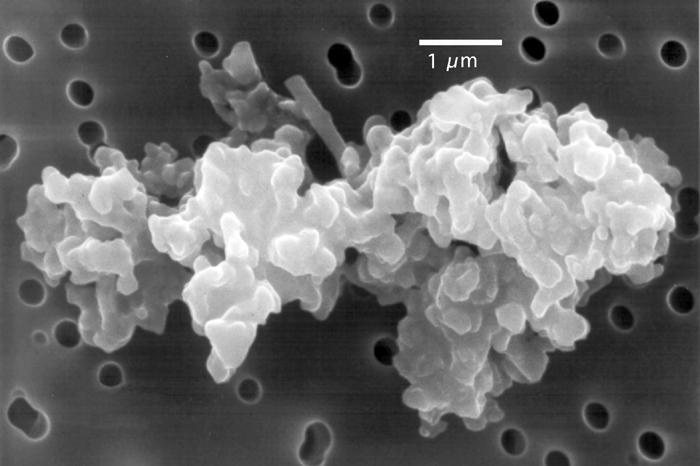
\includegraphics[width=8cm]{figures/grain.jpg}
 	\caption{A scanning electron microscopy (\textit{SEM}) image of a porous chondrite dust grain recovered from high atmosphere.  The authors of this figure are Donald E. Brownlee, University of Washington, Seattle, and Elmar Jessberger, Institut für Planetologie, Münster, Germany.
This file is licensed under CC-BY 2.5 License.}
 	\label{fig:dust_grain}
\end{figure}

\subsection{Dust density} \label{sec:density}

Bulk density of the common minerals containing the usual meteorite component elements, such as \textit{olivine}, \textit{quartz} or \textit{pyroxenes} is between $2.6 \, \si{g cm^{-3}}$ and $3.8 \, \si{g cm^{-3}}$ \citep{duda1986minerals}. A lot of interplanetary dust contains ice, which naturally has a bulk density close to $1 \, \si{g cm^{-3}}$.

The density is often assumed between $2.5 \, \si{g cm^{-3}}$ \citep{mann2014dust} and $3 \, \si{g cm^{-3}}$ \citep{mcdonnell1984cosmic}. Dust grains are often, due to photometric and historical reasons described in terms of their linear dimension $d = 2r$, which more often than not means the diameter of the sphere with the volume $V$ equivalent to the dust grain's, hence

\begin{equation}
    d = 2 \left( {\frac{3V}{4\pi}} \right)^{\frac{1}{3}} \approx 1.24 \sqrt[3]{V}.
\end{equation}

Since we meet both mass-based notation and size-based notation, it is useful to keep the conversion in mind, which stands

\begin{equation}
    m = \rho \frac{4\pi}{3} r^3 = \rho \frac{\pi}{6} d^3 \Leftrightarrow d = \sqrt[3]{\frac{6 m}{\rho \pi}},
    \label{eq:density}
\end{equation}

and assuming $2.5 \, \si{g cm^{-3}}$ gives

\begin{equation}
    \frac{m}{\si{kg}} \approx 1.3 \cdot 10^3 \left(\frac{d}{\si{m}}\right)^3 
\Leftrightarrow 
    \frac{d}{\si{m}} = 9 \cdot 10^{-2} \sqrt[3]{\frac{m}{\si{kg}}},
\end{equation}

which is shown in \Figref{fig:mass_size_ruler}.

\begin{figure}[h]
 	\centering
 	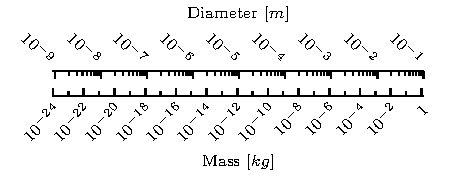
\includegraphics[width=10cm]{figures/mass_size_ruler.pdf}
 	\caption{A conversion between the mass and the diameter of a spherical dust grain, assuming the density of $2.5 \, \si{g cm^{-3}}$.}
 	\label{fig:mass_size_ruler}
\end{figure}

\section{Gravity} \label{ch:gravity}

Gravity is an attractive pair force between two heavy objects of the magnitude of 

\begin{equation}
    F_g = G \frac{M m}{R^2} = \mu \frac{m}{R^2},
\end{equation}

where $G \approx 6.67 \cdot 10^{-11} m^3 kg^{-1} s^{-2}$ is the \textit{gravitational constant}, $R$ is the distance between the objects' centres of mass, and masses $M$ and $m$ belong, by convention, to the more and less massive of the objects, respectively. Alternatively, $\mu = G M$ is known as the \textit{gravitational parameter}, which provides a convenient form for the force, especially if $m \ll M$, as is certainly the case of dust grains, with respect to planets and the Sun. In case of the Sun, $\mu \approx 1.3 \cdot 10^{20} \si{m^3 s^{-2}}$.

Due to the steep dependence of the force on the distance $F_g \propto R^{-2}$, it is often the case that a single central body suffices to describe the net gravity force affecting a smaller body. This concept is known as the \textit{Hill sphere}, which is the sphere of influence around every body in the Solar system, within which the body's gravity is the most relevant contributor to the net gravity, compared against the gravity of the Sun. The approximate planet's Hill radius is equal to the distance to the $L_1$ or the $L_2$ Lagrange point, therefore 

\begin{equation}
    R_H \approx a \sqrt[3]{\frac{m}{3M}},
\end{equation}

where $a$ is the planet's semimajor axis, $m$ is the mass of the planet, and $M$ is the mass of the Sun \cite{sheppard2023new}. For example, Saturn's Hill sphere with the Hill radius of $R_{H;Saturn} \approx 0.4 \, \si{AU}$ is necessary for Saturn to retain is $146$ confirmed moons \citep{sheppard2023new}, as well as its far reaching rings. The rings are an example of a dust system bound to a planet, as well as, in the case of Saturn's E-ring, a moon \citep{kempf2010enceladus}. Earth has the biggest Hill sphere of all the inner planets, $R_{H;Earth} \approx 10^{-2} \, \si{AU}$. The dust does not have be present inside a planet's Hill sphere to be influenced by its gravity, as Jupiter's Trojans prove, concentrated around its $L_4$ and $L_5$ Lagrange points. The Sun is however the dominant object in most of the Solar system, especially within $1 \, \si{AU}$.

Many object in the Solar system orbit on approximately circular orbits. Such orbit occurs if the magnitude of centrifugal force $F_c$ is equal to the magnitude of gravity $F_g$. The centrifugal force magnitude is 

\begin{equation}
    F_c = \frac{m v^2}{R}, 
\end{equation}
where $R$ is the curvature radius and $v$ is the orbital speed. The $v_c$ needed for the equality $F_c = F_g$ is then

\begin{equation}
    \frac{m v_c^2}{R} = \mu \frac{m}{R^2} \Leftrightarrow v_c = \sqrt{\frac{\mu}{R}}.
    \label{eq:circular_speed}
\end{equation}
The circular speed $v_c$ at $R = 1 \, \si{AU}$ is $v \approx 29.8 \, \si{km s^{-1}}$. 

The work $W$ done against the gravity during motion in the solar gravity field is

\begin{equation}
    W = \int_{l} \vec{F_g} \cdot \, d\vec{s} = \mu m \left( \frac{1}{R_0} - \frac{1}{R_1} \right)
\end{equation}
where $l$ is the trajectory of the motion, $R_0$ is the starting heliocentric distance and $R_1$ is the final heliocentric distance. Since gravity ceases as $R \to \infty$ quickly enough ($F_g \propto R^{-2}$), the work $W_e$ needed in order to escape the gravity of the Sun from the heliocentric distance $R$ finite:

\begin{equation}
    W_e =  \frac{\mu m}{R}.
\end{equation}
If the energy to do the work $W_e$ comes from the kinetic energy $E_k$ of the object,

\begin{equation}
    E_k = \frac{m v^2}{2},
\end{equation}
then the condition for speed $v_e$ to provide sufficient energy is

\begin{equation}
    \frac{m v_e^2}{2} = \frac{\mu m}{R} \Leftrightarrow v_e = \sqrt{\frac{2 \mu}{R}},
    \label{eq:escape_speed}
\end{equation}
where $v_e$ is called the \textit{escape speed}. We note that 

\begin{equation}
    v_e = \sqrt{2} v_c.
\end{equation}


\section{Radiation pressure}

The power density of solar radiation at $1 \si{AU}$ is $G_{SC} \approx 1361 \, \si{W m^{-2}}$ \citep{kopp2011new} and corresponds to the radiative power of the Sun $P_{Sun} \approx 3.9 \cdot 10^{26} \, \si{W}$. Dividing $G_{SC}$ by the speed of light $c \approx 3\cdot10^8 \, \si{m s^{-1}}$ gives the radiation pressure of

\begin{equation}
    p_{RP}(1 \si{AU}) = \frac{G_{SC}}{c} \approx 4.5 \cdot 10^{-6} \, \si{Pa},
\end{equation}
and the resulting radiation pressure force $F_{RP}$ is readily obtained as

\begin{equation}
    F_{RP} = p_{RP} S = \frac{P_{Sun}}{4 c \pi R^2} S = \frac{P_{Sun}}{cR^2} r^2, \label{eq:radiation_pressure_force}
\end{equation}
where $S$ is the Sun-facing cross section of the body of interest, $r$ is the body's radius, and $R$ is the distance of the body from the Sun, whereas in the second equation we also assumed the body to be spherical and the Sun to be a point source: $r \ll R$. A dimensionless parameter $\beta$ is used to describe the relative importance of the two forces:

\begin{equation}
    \beta = \frac{F_{RP}}{F_g}.
\end{equation}
Since $F_{RP}$ directly opposes $F_g$, the net force, denoted \textit{effective gravity}, or $F_{eg}$ is obtained as

\begin{equation}
    F_{eg} = F_g - F_{RP},
\end{equation}
and using $\beta$, we get

\begin{equation}
    F_{eg} = (1-\beta) F_g.
\end{equation}
In the case of the Earth, the radiation pressure force is $F_{RP;Earth} \approx 5.8 \cdot 10^8 \, \si{N}$, which might be compared to the gravity between the Earth and the Sun $F_{g;Earth} \approx 5.2 \cdot 10^{33} \si{N}$, resulting in $\beta_{Earth} \approx 10^{-25}$. 

Interestingly, both $F_g$ and $F_{RP}$ scale with the distance from the Sun as $F \propto {R^-2}$, as long as the Sun is assumed a point source of radiation. Therefore, $\beta$ is not a function of the distance from the Sun $R$, and we are permitted to express the effective gravity as 

\begin{equation}
    F_{eg} = (1-\beta) G \frac{M m}{R^2} = (1-\beta) \mu \frac{m}{R^2} = \mu_{e} \frac{m}{R^2},
\end{equation}

where $\mu_{e}$ is the body-specific effective gravitational parameter, taking radiation pressure into account. We see that the laws of orbital motion (for example Eqs. \ref{eq:circular_speed} and \ref{eq:escape_speed}) of radiation pressure affected bodies are going to be the same, albeit with a different gravitational parameter $\mu_e$.

We found that $\beta$ only depends on the properties of the Sun and the body in question, and is therefore body specific. Let us study the dependence of $\beta$ on the size of the body in question $r$. It follows that as long as the aforementioned equations for $F_{g}$ and $F_{RP}$ hold, $\beta$ depends on $r$ as 

\begin{equation} 
    \beta = \frac{\frac{P_{Sun}}{c R^2} r^2}{\mu \frac{m}{R^2}} = \frac{P_{Sun}}{\mu c} \frac{r^2}{\rho V} = \frac{P_{Sun}}{\mu c \rho} \frac{3 r^2}{4 \pi r^3} = \frac{3 P_{Sun}}{4 \pi \mu c \rho} r^{-1},
\end{equation}

therefore $\beta \propto r^{-1}$, which is not surprising, given $F_{g} \propto m \propto r^{3}$ and 
$F_{RP} \propto S \propto r^{2}$. Assuming the density of $\rho \approx 2.5 \si{gcm^{-3}}$ as in Sec. \ref{sec:density}, we find that 

\begin{equation}
    \beta \approx 9.5 \cdot 10^{-7} r^{-1},
\end{equation}

which gives that for $\beta = 1$, that is the radiation pressure force offsetting the gravity fully, the dust grain has to have the radius of $r \approx 950 \, \si{nm}$. However, Eq. \eqref{eq:radiation_pressure_force} assumes the solar photons are either absorbed, or scattered fully as a spherical wave --- their momentum transferred to the body. This holds for absorbing materials if $r \gg \lambda$, where $\lambda$ is the wavelength of the radiation. However, $r \approx 950 \si{nm}$ is comparable to the typical sunlight photons and the assumption does not hold fully. A proper calculation of \textit{Mie scattering} is necessary and it depends on the material and shape of the grain. This was done previously by other authors \cite{kimura2003composition} for reasonable materials. It was found that the maximum of $\beta$ is reached between $10^{-17} - 10^{-16} \si{kg}$, which corresponds to the diameter of $100 - 300 \si{nm}$, depending on the material. In any case, the maximum value of $\beta$ is on the order of unity and lower than unity for much smaller or larger grains.

\begin{figure}[h]
 	\centering
 	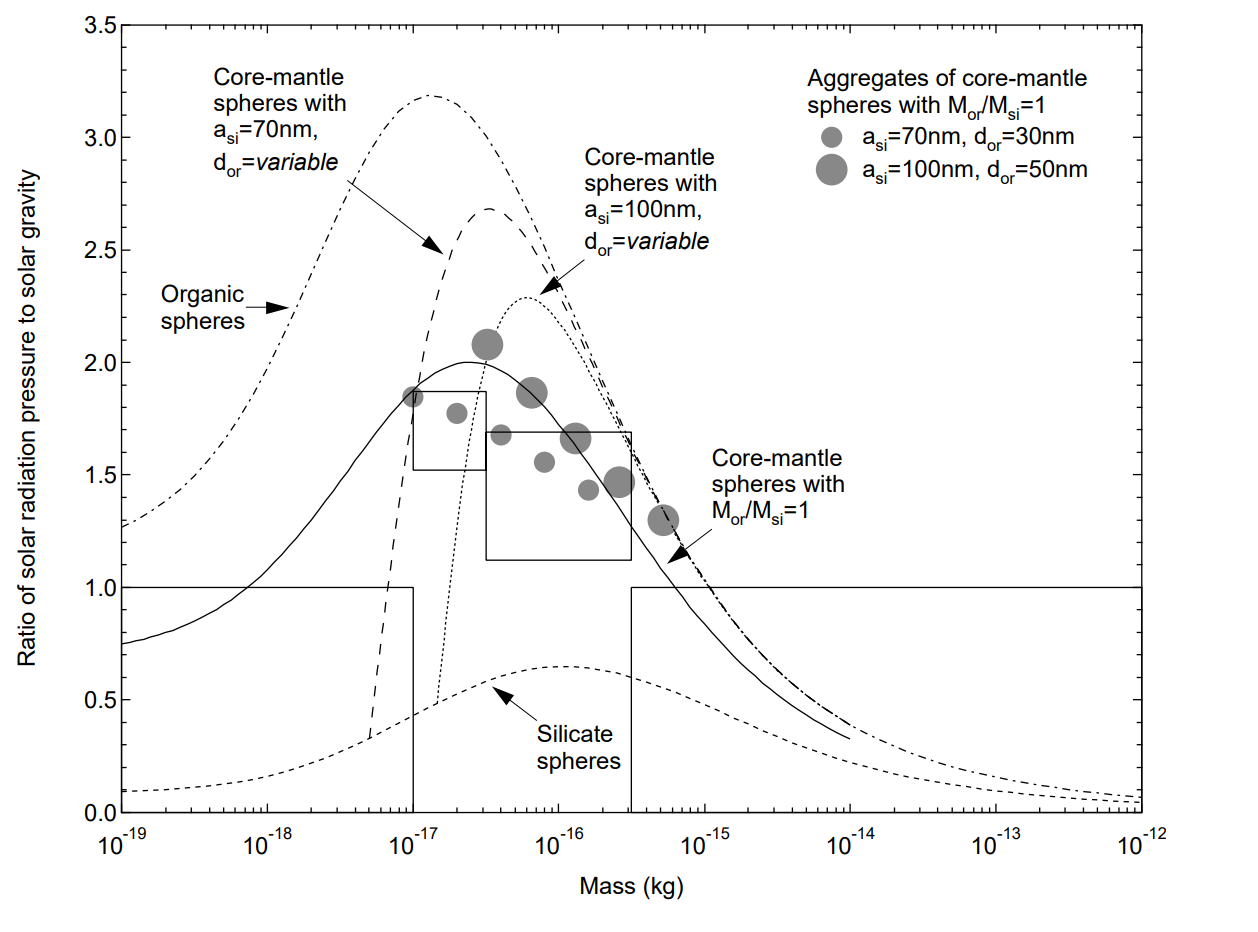
\includegraphics[width=10cm]{figures/kimurra_mie.png}
 	\caption{The Mie theory result for the $\beta$ value (\textit{y}-axis) as a function of mass of spherical grains of various composition, adapted from \cite{kimura2003composition}.}
 	\label{fig:kimura_mie}
\end{figure}

\section{Lorentz force}

\subsection{Grain's potential}

The grains in the solar system are immersed in the ambient plasma and subjected to the solar UV irradiation, both of these causing charging of the grains. Should the ambient conditions remain stable, the grain's electric charge reaches equilibrium. The main charging currents are \textit{electron collection current} and the \textit{photoemission current}. They act to charge the grain to a negative and positive potential respectively. Should the plasma be dense or should the grain be in shadow, the former prevails and the grain's potential becomes negative. Should the plasma be sparse and the UV irradiation dense, the latter prevails and the grain becomes positively charged. We will now examine the two extreme cases. 

An object immersed in plasma charges to so-called \textit{floating potential}. This potential $\phi_{f}$ is typically negative, which is a result of the electron mobility being much higher, compared to the ion mobility. The charging current ceases if the potential of the grain poses a significant barrier to the electrons, therefore the maximum potential is on the order of electron temperature $T_e$, which is approximately $8 \, \si{eV k_B^{-1}}$ near $1 \, \si{AU}$ and $20 \, \si{eV k_B^{-1}}$ near $0.25 \, \si{AU}$ in the typical solar wind \citep{guillemant2013simulation}. 

Electrons are released from an illuminated neutral grain, in case the incident photon's energy $h\nu$ is above the photoelectric work function $W_{p}$ of the grain material. This typically requires UV photons and leaves the grain more positively charged, which adds additional barrier for the next photoelectron to surpass. The established positive potential $\phi_{p}$ is such that no more electrons can escape, therefore it is $\phi_{p} \approx h\nu - W_{p}$. While $W_p$ for common materials is between $2 - 5 \, \si{eV}$, the last strong spectral line of she sunlight is \textit{Ly-$\alpha$} at $h\nu \approx 10.2 \, \si{eV}$, resulting in the maximum potential of $\phi_p$ between $5 - 8 \, \si{V}$. 

The equilibrium potential $\phi$ of the grain depends on the ambient plasma conditions and the properties of the grain, but typically settles on a value between $-20 \, \si{V}$ and $+8 \, \si{V}$. 

\subsection{Grain's charge}

An isolated grain's charge $q$ is related to its potential $\phi$ as

\begin{equation}
    q = C \phi, \label{eq:charge}
\end{equation}

where $C$ is the grain's capacitance. The capacitance of a solitary sphere in vacuum with the radius of $r$ is 

\begin{equation}
    C_{sphere} = 4 \pi \epsilon_0 r,
\end{equation}

which translates using Eq. \ref{eq:charge} to

\begin{equation}
    \frac{q}{r \phi} = 4 \pi \epsilon_0 \approx 1.1 \cdot 10^{-10} \, \si{C V^{-1} m^{-1}},
    \label{eq:capacitance}
\end{equation}

where $\epsilon_0 \approx 8.9\cdot10^{-12} \, \si{C V^{-1} m^{-1}}$ is the free space permittivity. This simplistic model predicts the charge of $\pm 10^{-15} \, \si{C}$ for a spherical grain with the radius of $r = 1 \, \si{\mu m}$ at the potential of $\phi = \pm 9 \, \si{V}$. We note that this value is order of magnitude correct for a grain of arbitrary shape with the greatest linear extent of $\approx 2r$.

\subsection{Dynamics}

Considering the scale of the Solar system, a point charge is a very suitable model for a charged dust grain. The Lorentz force acting on a point charge $q$ is

\begin{equation}
\vec{F}_{EM} = q \left( \vec{E} + \vec{v} \times \vec{B} \right),
\end{equation}

where $\vec{E}$ and $\vec{B}$ are the ambient electric and magnetic fields respectively, and $\vec{v}$ is the velocity of the point charge. If the charge $q$ is sufficient, $F_{EM}$ might be more important than effective gravity:

\begin{equation}
    F_eg < F_{EM} \Rightarrow \frac{q}{m} > \frac{(1-\beta)\mu}{R^2 \left| \vec{E} + \vec{v} \times \vec{B} \right|}. \label{eq:lorentz_gravity}
\end{equation}

This condition describes the state in which the Lorentz force is grater in amplitude than the gravity. Mind that if they are equal, the curvature in the trajectory of the dust grain due to the Lorentz force is similar to the curvature of the trajectory due to the force of gravity, which is on the Solar system scale. It is therefore important to consider the temporal aspect: given enough time, even $F_{EM} \ll F_g$ might be consequential for the motion of the dust grain, and, vice-versa, $F_{EM} \approx F_g$ does not imply that the grain does not move along a straight line when inspected locally. It is also apparent that this condition has many degrees of freedom. We are now going to examine two relevant cases: a) dust near the Earth immersed in the solar wind, and b) dust in the solar F-corona. More extensive discussion is outside of the scope of this work, but numerous publications dive in the topic of the motion of charged grains immersed in the solar system plasma \citep{mann2007nanoparticles,stamm2019dust,czechowski2021dynamics,poppe2022effects}, as well as the grain charging processes \citep{meyer1982flip,vaverka2016lunar}.

\subsubsection{Dust near the Earth immersed in the solar wind}

Due to solar wind's very high conductance, there is very little intrinsic electric field in the interplanetary medium. Ihe interplanetary magnetic field (\textit{IMF}, $\vec{B}_{IMF}$) is in so-called \textit{forzen-in} state and approximately follows the Parker spiral \citep{parker1958dynamics}. One of the consequences is that the IMF near the solar equator near the Sun ($R \ll 1 \, \si{AU}$) is predominantly radial, whereas far from the Sun ($R \gg 1 \, \si{AU}$) it is predominantly azimuthal. Near $1 \, \si{AU}$, the IMF is directionally variable, with the typical strength of $B_{IMF} \approx 4 \, \si{nT}$ \citep{mann2007nanoparticles}. This magnetic field is  embedded in the parcels of solar wind, moving with the velocity of $\vec{v_{sw}}$ in the heliocentric frame. The typical solar wind speed of $v_{sw} \approx 300 \, \si{km s^{-1}}$ is much higher than the orbital speed of the Earth $v_{Earth} \approx 30 \, \si{km s^{-1}}$. The modulus of the resulting Lorentz force is then approximately 

\begin{equation}
    F_{EM} \approx q v_{sw} B_{IMF},
\end{equation}
which gives the condition \ref{eq:lorentz_gravity} the form of

\begin{equation}
    \frac{q}{m} > \frac{(1-\beta)\mu}{R^2 v_{sw} B_{IMF}},
\end{equation}
which is, assuming $\beta = 0$, $R = 1 \, \si{AU}$, $\mu$ as in Sec. \ref{ch:gravity}, and $B_{IMF}$, $v_{sw}$ as in the current section:

%\begin{equation}
%    \frac{q}{m} > \frac{1.3 \cdot 10^{20} \, \si{m^3 s^{-2}}}{1.5^2 \cdot 10^{22} \si{m^2} \, 3 \cdot 10^5 \, \si{ms^{-1}} \, 4 \cdot 10^{-9} \, \si{T}} \approx 4.8 \, \si{C kg^{-1}}.
%\end{equation}
\begin{equation}
    \frac{q}{m} >  4.8 \, \si{C kg^{-1}}.
\end{equation}
Given the charge as in Eq. \ref{eq:capacitance}, and the mass as in Eq. \ref{eq:density}, we get

\begin{equation}
    \frac{q}{m} = \frac{2 \epsilon_0 \phi}{\rho r^2}.
\end{equation}
Assuming the spherical grain's potential $\phi \approx 9 \, \si{V}$ and the bulk density $\rho \approx 2.5 \, \si{g cm^{-3}}$ as before, the condition \ref{eq:lorentz_gravity} states that 

\begin{equation}
    \frac{2 \epsilon_0 \phi}{\rho r^2} > \frac{(1-\beta)\mu}{R^2 v_{sw} B_{IMF}} \Leftrightarrow 
    r < \sqrt{\frac{2 \epsilon_0 \phi R^2 v_{sw} B_{IMF}}{(1-\beta) \mu \rho}} \approx 
    1.2 \cdot 10^{-7} \si{m}.
    \label{eq:nanodust_size_estimate}
\end{equation}

\subsubsection{Dust in the solar F-corona}

Solar F-corona is the corona region which gets the luminance from scattering the sunlight on the present dust grains. Further away from the Sun, F-corona smoothly transitions to zodiacal light. The Parker Solar Probe's closest \textit{sun-kissing} solar encounter, which is going to happen on the Christmas eve of 2024, will be just under $10 \, R_{Sun} \approx 0.046 \, \si{AU}$. Let us focus on this heliocentric distance as a model example. 

\citeauthor{guillemant2013simulation} conducted a particle-in-cell modelling study of the charging currents in several heliocentric locations \citep{guillemant2013simulation} spanning from $0.044 \, \si{AU}$ to $1 \, \si{AU}$. We will focus on $R = 0.044 \, \si{AU}$, as it nearly perfectly coincides with the Parker Solar Probe's closest perihelion. On that heliocentric distance, the magnetic field magnitude of $B_{IMF} = 2.1 \cdot 10^{-6} \, \si{T}$, along with other assumptions on the local plasma environment led to the floating potential of $\phi \approx -16 \, \si{V}$ \citep{guillemant2013simulation}. Making use of Eq. \ref{eq:circular_speed}, the circular speed $v_c$ at $R = 0.44 \, \si{AU}$ is $v_c \approx 142 \, \si{km s^{-1}}$, and this is the speed of the grain we use in the estimate. Using Eq. \ref{eq:nanodust_size_estimate}:

\begin{equation}
    r < \sqrt{\frac{2 \epsilon_0 \phi R^2 v_{c} B_{IMF}}{(1-\beta) \mu \rho}} \approx 
    1.1 \cdot 10^{-7} \si{m},
\end{equation}
which is very close to the result for dust near $1 \, \si{AU}$.

\section{Poynting-Robertson drag}

Since an object orbiting the Sun is moving with respect to the source of radiation, the position of the Sun as seen from the object is apparently different, \textit{aberrated}, by an angle of the order of $v/c$, where $v$ is the orbital speed of the object, and $c$ is the speed of light. Therefore, the light comes from the \textit{ram direction}, as observed from the orbiting object. The scattering and absorption of the light then leads to a negative change in the momentum, and therefore in the orbital speed \citep{poynting1903radiation}. The magnitude of Poynting-Robertson effect is \citep{robertson1937dynamical}:

\begin{equation}
    F_{PR} = \frac{v}{c^2} P_{r},
\end{equation}
where $P_r$ is the power of incoming solar radiation. Assuming the object on a circular orbit, we make use of Eq. \ref{eq:circular_speed}. Assuming the radiation power as in Eq. \ref{eq:radiation_pressure_force}, we get:

\begin{equation}
    F_{PR} = \sqrt{\frac{\mu}{R}} \frac{P_{r}}{c^2} = \frac{P_{Sun}}{4 \pi c^2} \sqrt{\frac{\mu}{R^5}} 
\end{equation}

TBD timescale estimate throught acceleration

\section{Yarkovsky effect}

only if I have nothing better to do

\section{Erosion}

sublimation, sputtering

\section{Collisions}

crushing law